\documentclass[]{article}
\usepackage{lmodern}
\usepackage{amssymb,amsmath}
\usepackage{ifxetex,ifluatex}
\usepackage{fixltx2e} % provides \textsubscript
\ifnum 0\ifxetex 1\fi\ifluatex 1\fi=0 % if pdftex
  \usepackage[T1]{fontenc}
  \usepackage[utf8]{inputenc}
\else % if luatex or xelatex
  \ifxetex
    \usepackage{mathspec}
  \else
    \usepackage{fontspec}
  \fi
  \defaultfontfeatures{Ligatures=TeX,Scale=MatchLowercase}
\fi
% use upquote if available, for straight quotes in verbatim environments
\IfFileExists{upquote.sty}{\usepackage{upquote}}{}
% use microtype if available
\IfFileExists{microtype.sty}{%
\usepackage{microtype}
\UseMicrotypeSet[protrusion]{basicmath} % disable protrusion for tt fonts
}{}
\usepackage[margin=1in]{geometry}
\usepackage{hyperref}
\hypersetup{unicode=true,
            pdftitle={Tema 1},
            pdfborder={0 0 0},
            breaklinks=true}
\urlstyle{same}  % don't use monospace font for urls
\usepackage{graphicx,grffile}
\makeatletter
\def\maxwidth{\ifdim\Gin@nat@width>\linewidth\linewidth\else\Gin@nat@width\fi}
\def\maxheight{\ifdim\Gin@nat@height>\textheight\textheight\else\Gin@nat@height\fi}
\makeatother
% Scale images if necessary, so that they will not overflow the page
% margins by default, and it is still possible to overwrite the defaults
% using explicit options in \includegraphics[width, height, ...]{}
\setkeys{Gin}{width=\maxwidth,height=\maxheight,keepaspectratio}
\IfFileExists{parskip.sty}{%
\usepackage{parskip}
}{% else
\setlength{\parindent}{0pt}
\setlength{\parskip}{6pt plus 2pt minus 1pt}
}
\setlength{\emergencystretch}{3em}  % prevent overfull lines
\providecommand{\tightlist}{%
  \setlength{\itemsep}{0pt}\setlength{\parskip}{0pt}}
\setcounter{secnumdepth}{0}
% Redefines (sub)paragraphs to behave more like sections
\ifx\paragraph\undefined\else
\let\oldparagraph\paragraph
\renewcommand{\paragraph}[1]{\oldparagraph{#1}\mbox{}}
\fi
\ifx\subparagraph\undefined\else
\let\oldsubparagraph\subparagraph
\renewcommand{\subparagraph}[1]{\oldsubparagraph{#1}\mbox{}}
\fi
%%%%%%%%%%%%%%%%%%%%%%%%%%%%%%%%%%%%%%%%%%%%%%%%%%%%%%%%%%%%%%%%%%%%%%%%%%%%%%%%%%%%%%%%%%%%%%%%%%%%%%%%%%%%%%%%%%%%%
%%%%%%%%%%%%%%%%%%%%%%%%%%%%%%%%%%%%%%%%%%%%%%%%%%%%%%%%%%%%%%%%%%%%%%%%%%%%%%%%%%%%%%%%%%%%%%%%%%%%%%%%%%%%%%%%%%%%%
%CITEVA DEFINITII
\def\om{\omega}
\def\Om{\Omega}
\def\et{\eta}
\def\td{\tilde{\delta}}
\def\m{{\mu}}
\def\n{{\nu}}
\def\k{{\kappa}}
\def\l{{\lambda}}
\def\L{{\Lambda}}
\def\g{{\gamma}}
\def\a{{\alpha}}
\def\e{{\varepsilon}}
\def\b{{\beta}}
\def\G{{\Gamma}}
\def\d{{\delta}}
\def\D{{\Delta}}
\def\t{{\theta}}
\def\s{{\sigma}}
\def\S{{\Sigma}}
\def\z{{\zeta}}
\def\qed{\hfill\Box}
\def\ds{\displaystyle}
\def\mc{\mathcal}
%%%%%%%%%%%%%%%%%%%%%%%%%%%%%%%%%%%%%%%%%%%%%%%%%%%%%%%%%%%%%%%%%%%%%%%%%%%%%%%%%%%%%%%%%%%%%%%%%%%%%%%%%%%%%%%%%%%%%%
\def\1{{\mathbf 1}}
\def\CC{{\mathbb C}}
\def\VV{{\mathbb V}}
\def\RR{{\mathbb R}}
\def\QQ{{\mathbb Q}}
\def\ZZ{{\mathbb Z}}
\def\PP{{\mathbb P}}
\def\EE{{\mathbb E}}
\def\NN{{\mathbb N}}
\def\FF{{\mathbb F}}
%\def\SS{{\mathbb S}}
\def\MA{{\mathcal A}}
\def\MO{{\mathcal O}}
\def\MF{{\mathcal F}}
\def\MR{{\mathcal R}}
\def\MB{{\mathcal B}}
\def\MM{{\mathcal M}}
\def\MN{{\mathcal N}}
\def\MU{{\mathcal U}}
\def\MP{{\mathcal P}}
\def\MS{{\mathcal S}}
\def\MBS{{\mathbf S}}
\def\MX{{\bm{ \mathscr X}}}
%%%%%%%%%%%%%%%%%%%%%%%%%%%%%%%%%%%%%%%%%%%%%%%%%%%%%%%%%%%%%%%%%%%%%%%%%%%%%%%%%%%%%%%%%%%%%%%%%%%%%%%%%%%%%%%%%%%%%
%Header and Footer
\usepackage{fancyhdr}

\pagestyle{fancy}
\fancyhf{}
\rhead{Universitatea din Bucure\c sti\\ Facultatea de Matematic\u a \c si Informatic\u a}
\lhead{\textit{Curs}: Probabilit\u a\c ti \c si Statistic\u a\\ \textit{Instructori}: A. Am\u arioarei, G. Popovici}
\rfoot{Pagina \thepage}
\lfoot{Grupele: 241, 242, 243, 244}
%%%%%%%%%%%%%%%%%%%%%%%%%%%%%%%%%%%%%%%

%%% Use protect on footnotes to avoid problems with footnotes in titles
\let\rmarkdownfootnote\footnote%
\def\footnote{\protect\rmarkdownfootnote}

%%% Change title format to be more compact
\usepackage{titling}

% Create subtitle command for use in maketitle
\newcommand{\subtitle}[1]{
  \posttitle{
    \begin{center}\large#1\end{center}
    }
}

\setlength{\droptitle}{-2em}
  \title{Tema 1}
  \pretitle{\vspace{\droptitle}\centering\huge}
  \posttitle{\par}
\subtitle{Soluții}
  \author{}
  \preauthor{}\postauthor{}
  \date{}
  \predate{}\postdate{}

\begin{document}
\maketitle

%%%%%%%%%%%%%%%%%%%%%%%%
\thispagestyle{fancy}

\subsubsection{\texorpdfstring{Exerci\c tiul
1}{Exerciiul 1}}\label{exerciiul-1}

\begin{enumerate}
\def\labelenumi{\alph{enumi})}
\item
  \(A\) singur se realizeaz\u a: \(A\cap B^c\cap C^c\)
\item
  \(A\) \c si \(C\) se realizeaz\u a dar nu \c si \(B\):
  \(A\cap B^c\cap C\)
\item
  cele trei evenimente se produc: \(A\cap B\cap C\)
\item
  cel pu\c tin unul dintre cele trei evenimente se produce:
  \(A\cup B\cup C\)
\item
  cel pu\c tin dou\u a evenimente din cele trei se produc:
  \(\left(A^c\cap B\cap C\right)\cup\left(A\cap B^c\cap C\right)\cup\left(A^c\cap B\cap C^c\right)\cup\left(A\cap B\cap C\right)\)
\item
  cel mult un eveniment se produce:
  \(\left(A^c\cap B^c\cap C\right)\cup\left(A^c\cap B\cap C^c\right)\cup\left(A\cap B^c\cap C^c\right)\cup\left(A^c\cap B^c\cap C^c\right)\)
\item
  niciunul din cele trei evenimente nu se produce:
  \(A^c\cap B^c\cap C^c\)
\item
  exact dou\u a evenimente din cele trei se produc:
  \(\left(A^c\cap B\cap C\right)\cup\left(A\cap B^c\cap C\right)\cup\left(A^c\cap B\cap C^c\right)\)
\item
  nu mai mult de dou\u a evenimente nu se realizeaz\u a:
  \(\left(A\cap B\cap C\right)^c\)
\end{enumerate}

\subsubsection{\texorpdfstring{Exerci\c tiul
2}{Exerciiul 2}}\label{exerciiul-2}

\begin{enumerate}
\def\labelenumi{\alph{enumi})}
\item
  ``so\c tul are mai mult de 40 de ani dar nu \c si so\c tia sa'' =
  \(A\cap C^c\)
\item
\end{enumerate}

\begin{itemize}
  
    \item $A\cap B\cap C^{c}=\{\mbox{ so\c tul are mai mult de 40 de ani dar so\c tia are mai pu\c tin de 40 de ani }\}$, 
    
    \item $A\setminus{(A\cap B)}=\{\mbox{ so\c tul are mai mult de 40 de ani iar so\c tia lui este mai in varst\u a decat el }\}$,
    
    \item $A\cap B^{c}\cap C=\{\mbox{ b\u arbatul are mai mult de 40 de ani iar so\c tia lui este mai in varst\u a decat el }\}$,
    
    \item $A\cup B=\{\mbox{ sau b\u arbatul are mai mult de 40 de ani sau femia este mai tan\u ar\u a decat el }\}$
    
  \end{itemize}

\begin{enumerate}
\def\labelenumi{\alph{enumi})}
\setcounter{enumi}{2}
\tightlist
\item
  Avem
  \(A\cap C^c\subset\left(A\cap C^c\right)\cup\left(A\cap B\cap C\right)\cup\left(A^c\cap B\cap C^c\right)=B\)
\end{enumerate}

\subsubsection{\texorpdfstring{Exerci\c tiul
3}{Exerciiul 3}}\label{exerciiul-3}

\begin{enumerate}
\def\labelenumi{\alph{enumi})}
\item
  Reamintim c\u a \(d:X\times X\to \RR\) este o distan\c t\u a pe \(X\)
  dac\u a verific\u a urm\u atoarele propriet\u a\c ti:

  \begin{enumerate}
  \def\labelenumii{\roman{enumii})}
  \item
    \(d(x,y)\geq 0\) (pozitivitate)
  \item
    \(d(x,y)=d(y,x)\) (simetrie)
  \item
    \(d(x,y)=0 \iff x=y\)
  \item
    \(d(x,y)\leq d(x,z)+d(y,z)\) pentru orice \(x,y,z\in X\)
    (inegalitatea triunghiului)
  \end{enumerate}
\end{enumerate}

In cazul problemei noastre obsrv\u am c\u a \(d(A,B)\geq 0\) \c si c\u a
\(d(A,B)=d(B,A)\) deoarece \(A\triangle B=B\triangle A\). S\u a
presupunem acum c\u a \(d(A,B)=0\). Avem
\(A\triangle B=\left(A\cap B^c\right)\cup\left(A^c\cap B\right)\) iar
din \(\left(A\cap B^c\right)\cap\left(A^c\cap B\right)=\emptyset\)
rezult\u a c\u a \[
  \PP(A\triangle B)= \PP(A\cap B^c) + \PP(A^c\cap B)=0\Rightarrow \PP(A\cap B^c)=0\;\mbox{\c si}\;\PP(A^c\cap B)=0
\] de unde \(\PP(A)=\PP(A\cap B)=\PP(B)\) deci \(A=B\) (a.s.).

Fie \(A, B, C\in \MF\). Vrem s\u a ar\u at\u am c\u a
\(d(A,B)\leq d(A,C)+d(B,C)\). Consider\u am evenimentele elementare
\(A\cap B\cap C\), \(A^c\cap B\cap C\), \(A\cap B^c\cap C\),
\(A\cap B\cap C^c\), \(A^c\cap B^c\cap C\), \(A^c\cap B\cap C^c\) \c si
\(A\cap B^c\cap C^c\) \c. Avem urm\u atoarele descompuneri:

\begin{align*}
  A\triangle B &= \left(A\cap B^c\cap C\right)\cup\left(A\cap B^c\cap C^c\right)\cup\left(A^c\cap B\cap C\right)\cup\left(A^c\cap B\cap C^c\right)\\
  A\triangle C &= \left(A\cap B\cap C^c\right)\cup\left(A\cap B^c\cap C^c\right)\cup\left(A^c\cap B\cap C\right)\cup\left(A^c\cap B^c\cap C\right)\\
  B\triangle C &= \left(A\cap B\cap C^c\right)\cup\left(A^c\cap B\cap C^c\right)\cup\left(A\cap B^c\cap C\right)\cup\left(A^c\cap B^c\cap C\right).
\end{align*}

Observ\u am c\u a
\(A\triangle B\subset\left(A\triangle C\right)\cup\left(B\triangle C\right)\)
de unde

\[
  \PP(A\triangle B)\leq\PP\left(\left(A\triangle C\right)\cup\left(B\triangle C\right)\right)\leq\PP(A\triangle C)+\PP(B\triangle C)
\]

ceea ce arat\u a c\u a \(d\) este distan\c t\u a.

\begin{enumerate}
\def\labelenumi{\alph{enumi})}
\setcounter{enumi}{1}
\tightlist
\item
  Consider\u am evenimentele elementare disjuncte \(A\cap B\),
  \(A\cap B^c\), \(A^c\cap B\) \c si \(A^c\cap B^c\). Avem urm\u atoarea
  descompunere
\end{enumerate}

\begin{align*}
  A &= \left(A\cap B^c\right)\cup\left(A\cap B\right)\\
  B &= \left(A^c\cap B\right)\cup\left(A\cap B\right)
\end{align*}

de unde ob\c tinem c\u a

\[
  \PP(A)-\PP(B) = \PP(A\cap B^c)+\PP(A\cap B)-\PP(A^c\cap B)-\PP(A\cap B)
\]

ceea ce arat\u a c\u a

\[
  |\PP(A)-\PP(B)|\leq \PP(A\cap B^c)+\PP(A^c\cap B)=\PP(A\triangle B).
\]

\subsubsection{\texorpdfstring{Exerci\c tiul
4}{Exerciiul 4}}\label{exerciiul-4}

\begin{figure}[ht]
         \centerline{
          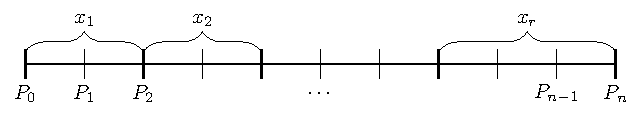
\includegraphics[width=0.6\textwidth]{Figs/fig_T1_ex4.pdf}}
          \caption{Interpretare geometric\u a}
          \label{fig_T1_ex4}
\end{figure}

\begin{enumerate}
\item Consider\u am un segment de dreapt\u a de lungime $n$ ca \c si in Fig.~\ref{fig_T1_ex4}. O solu\c tie $(x_1,x_2,\dots,x_r)$ a ecua\c tiei $x_1+\cdots+x_r=n$ astfel incat $x_i$ sunt numere intregi strict pozitive, corespunde unei descompuneri a acestui segment de dreapt\u a in $r$ p\u ar\c ti de lungime dat\u a de numere intregi strict pozitive. Cele $r-1$ puncte care determin\u a extremit\u a\c tile acestor segmente (altele decat $P_0$ \c si $P_n$) trebuie s\u a fie alese din cele $n-1$ puncte $P_1,P_2,\dots,P_{n-1}$ \c si acest lucru poate fi f\u acut in $\binom{n-1}{r-1}$ moduri diferite. Prin urmare num\u arul de solu\c tii strict pozitive ale ecua\c tiei $x_{1} + \ldots + x_{r} = n$ este $\binom{n-1}{r-1}$.

\item Fie $y_1=x_1+1$, $y_2=x_2+1$, $\dots$, $y_r=x_r+1$. Observ\u am c\u a $y_i$ sunt numere intregi strict pozitive \c si $y_1+y_2+\cdots+y_r=n+r$. Prin urmare num\u arul de solu\c tii intregi pozitive ale ecua\c tiei $x_{1} + \ldots + x_{r} = n$ este egal cu num\u arul de solu\c tii intregi strict pozitive ale ecua\c tiei $y_1+y_2+\cdots+y_r=n+r$ care am v\u azut c\u a este egal cu $\binom{n+r-1}{r-1}=\binom{n+r-1}{n}$.
\end{enumerate}

\subsubsection{\texorpdfstring{Exerci\c tiul
5}{Exerciiul 5}}\label{exerciiul-5}

\begin{enumerate}
\item
    \begin{enumerate}
        \item Spa\c tiul st\u arilor $\Om$ este $\Om=\{(O,b),(O,m),(O,s),(N,b),(N,m),(N,s)\}$.
        \item Avem
        \begin{align*}
            A &= \mbox{starea de s\u an\u atate a pacientului este serioar\u a} = \{(O,s),(N,s)\},\\
            B &= \mbox{pacientul nu este asigurat} = \{(N,b),(N,m),(N,s)\},\\
            B^{c}\cup A &= \mbox{sau pacientul este asigurat sau starea acestuia este serioas\u a}\\
                &= \{O,b),(O,m),(O,s),(N,s)\}.
        \end{align*}
    \end{enumerate}
\item Cum m\u asura de probabilitate $\PP$ corespunde echiprobabilit\u a\c tii pe $\Om$ avem c\u a $\PP((O,b))=\PP((O,m))=\PP((O,s))=\PP((N,b))=\PP((N,m))=\PP((N,s))=\frac{1}{6}$, deci
    \begin{align*}
            \PP(A) &= \PP((O,s))+\PP((N,s)) = \frac{1}{3},\\
            \PP(B) &= \PP((N,b))+\PP((N,m))+\PP((N,s)) = \frac{1}{2},\\
            \PP(B^c\cup A) &= \PP((O,b))+\PP((O,m))+\PP((O,s))+\PP((N,s)) = \frac{2}{3}.
    \end{align*}
\item In acest caz avem
    \begin{align*}
            \PP(A) &= \PP((O,s))+\PP((N,s)) = 0.1+0.1 = 0.2,\\
            \PP(B) &= \PP((N,b))+\PP((N,m))+\PP((N,s)) = 0.1+0.3+0.1 = 0.5,\\
            \PP(B^c\cup A) &= \PP((O,b))+\PP((O,m))+\PP((O,s))+\PP((N,s)) = 0.2+02+0.1+0.1 = 0.6.
    \end{align*}

\end{enumerate}

\subsubsection{\texorpdfstring{Exerci\c tiul
6}{Exerciiul 6}}\label{exerciiul-6}

\begin{enumerate}
\def\labelenumi{\alph{enumi})}
\item
  Careu:
  \(\frac{\binom{13}{1}\binom{12}{1}\binom{4}{1}}{\binom{52}{5}}=\frac{624}{2598960}=\)
  0.024\%
\item
  Full-house:
  \(\frac{\binom{13}{1}\binom{4}{3}\binom{12}{1}\binom{4}{2}}{\binom{52}{5}}=\frac{3744}{2598960}=\)
  0.14\%
\item
  Trei c\u ar\c ti de acela\c si tip:
  \(\frac{\binom{13}{1}\binom{4}{3}\binom{12}{2}\binom{4}{1}\binom{4}{1}}{\binom{52}{5}}=\frac{54912}{2598960}=\)
  2.1\%
\item
  Dou\u a perechi:
  \(\frac{\binom{13}{2}\binom{4}{2}\binom{4}{2}\binom{11}{1}\binom{4}{1}}{\binom{52}{5}}=\frac{123552}{2598960}=\)
  4.75\%
\item
  O pereche:
  \(\frac{\binom{13}{1}\binom{4}{2}\binom{12}{3}\left(\binom{4}{1}\right)^3}{\binom{52}{5}}=\frac{1098240}{2598960}=\)
  42.26\%
\end{enumerate}

\subsubsection{\texorpdfstring{Exerci\c tiul
7}{Exerciiul 7}}\label{exerciiul-7}

Consider\u am evenimentele urm\u atoare:

\begin{itemize}
  \item[-] $A=\{\mbox{testul considerat este pozitiv}\}$ 
  \item[-] $B=\{\mbox{automobilistul a dep\u a\c sit nivelul de alcool autorizat}\}$
\end{itemize}

\begin{enumerate}
    \item Din ipotez\u a \c stim c\u a $\PP(B) = 0.005$, $\PP(A|B) = \PP(A^c|B^c) = 0.99$. Vrem s\u a g\u asim probabilitatea $\PP(B|A)$. Avem
\begin{align*}
    \PP(B|A) &= \frac{\PP(A\cap B)}{\PP(B)} = \frac{\PP(A|B)\PP(B)}{\PP(B)} = \frac{\PP(A|B)\PP(B)}{\PP(A|B)\PP(B)+\PP(A|B^c)\PP(B^c)}\\
             &= \frac{\PP(A|B)\PP(B)}{\PP(A|B)\PP(B)+\left[1-\PP(A^c|B^c)\right](1-\PP(B))} = \frac{0.99\times0.005}{0.99\times0.005+0.01\times0.995} \approx 0.332.
\end{align*}
    \item C\u aut\u am $p$ a\c sa incat $\PP(B|A)=0.95$. Am v\u azut c\u a $\PP(B|A) = \frac{p\PP(B)}{p\PP(B)+(1-p)(1-\PP(B))}$ de unde
\begin{equation*}
    p = \frac{(1-\PP(B))\PP(B|A)}{(1-\PP(B))\PP(B|A)+(1-\PP(B|A))\PP(B)} = \frac{0.995\times0.95}{0.995\times0.95+0.05\times0.005}\approx0.99973.
\end{equation*}
    \item \c Stim c\u a $\PP(B)=0.3$, prin urmare $\PP(A) = \PP(A|B)\PP(B)+\PP(A|B^c)\PP(B^c) = 0.99\times0.3+0.01\times0.7\approx0.304$ \c si
\begin{equation*}
    \PP(B|A) = \frac{\PP(A|B)\PP(B)}{\PP(A|B)\PP(B)+\PP(A|B^c)\PP(B^c)}\approx 0.9769,
\end{equation*}
de unde tragem concluzia c\u a testul este mult mai fiabil in aceast\u a situa\c tie.
\end{enumerate}

\subsubsection{\texorpdfstring{Exerci\c tiul
8}{Exerciiul 8}}\label{exerciiul-8}

\begin{enumerate}
\item Consider\u am evenimentele urm\u atoare: 
  \begin{itemize}
    \item[-] $A_i=\{\mbox{suma celor dou\u a zaruri la cea de- a $i$-a aruncare este $5$}\}$
    \item[-] $B_i=\{\mbox{suma celor dou\u a zaruri la cea de- a $i$-a aruncare este $7$}\}$
  \end{itemize}  
Evenimentul $E_n$ se scrie
    \begin{equation*}
        E_n = (A_1^c\cap B_1^c)\cap(A_2^c\cap B_2^c)\cap\dots\cap(A_{n-1}^c\cap B_{n-1}^c)\cap A_n.
    \end{equation*}
Aplicand independen\c ta avem c\u a
    \begin{align*}
        \PP(E_n) &= \PP((A_1^c\cap B_1^c)\cap(A_2^c\cap B_2^c)\cap\dots\cap(A_{n-1}^c\cap B_{n-1}^c)\cap A_n)\\
                 &\overset{indep.}{=} \PP(A_1^c\cap B_1^c)\times \PP(A_2^c\cap B_2^c)\times\dots\times \PP(A_{n-1}^c\cap B_{n-1}^c)\times \PP(A_n)\\
                 &= \PP(A_1^c\cap B_1^c)^{n-1}\PP(A_n).
    \end{align*}
Observ\u am c\u a spa\c tiul st\u arilor la cea de-a $n$-a lansare este $\Om=\{(i,j)|1\leq i,j\leq6\}$ \c si probabilitatea ca suma celor dou\u a zaruri s\u a fie $5$ este $\PP(A_n) = \frac{4}{36}$, deoarece cazurile favorabile sunt $\{(1,4),(2,3),(4,1),(3,2)\}$. Ob\c tinem de asemenea c\u a probabilitatea ca suma s\u a nu fie nici $5$ \c si nici $7$ la prima lansare este $\PP(A_1^c\cap B_1^c) = \frac{26}{36}$, deoarece situa\c tiile in care suma este $7$ sunt $\{(1,6),(2,3),(3,4),(4,3),(5,2),(6,1)\}$.
\par \noindent
In concluzie, probabilitatea evenimentului 
$$
  A=\{\mbox{suma $5$ (a fe\c telor celor dou\u a zaruri) s\u a apar\u a inaintea sumei $7$}\}
$$ 
este 
\begin{align*}
    \PP(A) &= \displaystyle\PP\left(\bigcup_{n=1}^{\infty}E_n\right)=\sum_{n=1}^{\infty}\PP(E_n)=\sum_{n=1}^{\infty}\left(\frac{26}{36}\right)^{n-1}\frac{4}{36}\\
            &= \frac{1}{9}\sum_{n=0}^{\infty}\left(\frac{13}{18}\right)^{n} = \frac{1}{9}\frac{1}{1-\frac{13}{18}}=\frac{2}{5}.
\end{align*}
\item Fie $F_n$ evenimentul ce corespunde la: \textit{in primele $n-1$ arunc\u ari nu a ap\u arut nici suma $2$ \c si nici suma $7$ iar in a $n$-a aruncare a ap\u arut suma $2$} \c si $C_i$ evenimentul ce corespunde la suma celor dou\u a zaruri la cea de-a $i$-a aruncare este $2$. Avem
    \begin{equation*}
        F_n = (C_1^c\cap B_1^c)\cap(C_2^c\cap B_2^c)\cap\dots\cap(C_{n-1}^c\cap B_{n-1}^c)\cap C_n
    \end{equation*}
\c si probabilitatea lui $\PP(F_n)$ este
    \begin{align*}
        \PP(F_n) &= \PP((C_1^c\cap B_1^c)\cap(C_2^c\cap B_2^c)\cap\dots\cap(C_{n-1}^c\cap B_{n-1}^c)\cap C_n)\\
                 &\overset{indep.}{=} \PP(C_1^c\cap B_1^c)\times \PP(C_2^c\cap B_2^c)\times\dots\times \PP(C_{n-1}^c\cap B_{n-1}^c)\times \PP(C_n)\\
                 &= \PP(C_1^c\cap B_1^c)^{n-1}\PP(C_n).
    \end{align*}
Avem $\PP(C_n) = \frac{1}{36}$ (deoarece doar $(1,1)$ ne d\u a suma $2$) \c si $\PP(C_1^c\cap B_1^c) = \frac{36-7}{36} = \frac{29}{36}$. Prin urmare probabilitatea evenimentului c\u autat, pe care il not\u a cu $B$, este
\begin{align*}
    \PP(B) &= \displaystyle\PP\left(\bigcup_{n=1}^{\infty}F_n\right)=\sum_{n=1}^{\infty}\PP(F_n)=\sum_{n=1}^{\infty}\left(\frac{29}{36}\right)^{n-1}\frac{1}{36}\\
            &= \frac{1}{36}\sum_{n=0}^{\infty}\left(\frac{29}{36}\right)^{n} = \frac{1}{36}\frac{1}{1-\frac{29}{36}}=\frac{1}{7}.
\end{align*}
\end{enumerate}

\subsubsection[Exerci\c tiul 9*
\label{Ex6}]{\texorpdfstring{Exerci\c tiul 9* \footnote{Exerci\c tiile
  cu * sunt suplimentare \c si nu sunt obligatorii}
\label{Ex6}}{Exerciiul 9*  }}\label{exerciiul-9}

Fie parti\c tia
\(\Pi=\{A_1^{\e_1}\cap A_2^{\e_2}\cap\cdots\cap A_n^{\e_n}\,|\,\e_1,\dots,\e_n=0,1\}\),
unde \(A^{\e}=A\) dac\u a \(\e=1\) \c si \(A^{\e}=A^c\) dac\u a
\(\e = 0\). Atunci \(\MF=\MA(\{A_1,\dots, A_n\})\) (algebra generat\u a
de \(\{A_1,\dots,A_n\}\)) coincide cu algebra generat\u a de \(\Pi\),
prin urmare orice element din \(\MF\) poate fi scris ca o reuniune
finit\u a (\c si disjunct\u a) de elemente din \(\Pi\) (De ce?). Astfel,
pentru \(B_1, \dots, B_m\in\MF\) exist\u a \(\a_1,\dots,\a_{m'}\in\Pi\)
a\c sa incat s\u a avem \[
  \displaystyle\sum_{i=1}^{m}c_i\PP(B_i)=\sum_{i=1}^{m'}c'_{i}\PP(\a_i').
\] Este evident c\u a implica\c tia \(a)\implies b)\) este
adev\u arat\u a. Reciproc, s\u a presupunem c\u a inegalitatea dorit\u a
este adev\u arat\u a pentru orice m\u asur\u a de probabilitate cu
\(\PP(A_i)=0\) sau \(1\) pentru to\c ti \(i\in\{1,2,\dots,n\}\). Avem
deci c\u a

\begin{equation}\label{eqEx6}
  \sum_{i=1}^{m'}c'_{i}\PP(\a_i')\geq 0 
\end{equation}

pentru toate m\u asurile de probabilitate cu \(\PP(A_i)=0\) sau \(1\),
\(\forall\, i\in\{1,2,\dots,n\}\), prin urmare \(\PP(\a_i)=0\) sau \(1\)
pentru toate elementele \(\a_i\) din \(\Pi\) (to\c ti atomii). Alegand
\(P\) a\c sa incat \(\PP(\a_i)=1\), pentru un \(i\) fixat, \c si
\(\PP(\b)=0\) pentru \(\b\in\Pi, \, \b\neq\a\) \footnote{putem g\u asi o
  asemenea m\u asur\u a de probabilitate deoarece odat\u a ce am ales
  \(\PP(\a_i)=1\) am ales \c si valorile pentru \(\PP(A_j)\)} avem
\(c'_i\geq 0\) (\(i=1,2\dots,m'\)). Asta garanteaz\u a c\u a rela\c tia
(\ref{eqEx6}) r\u amane valabil\u a pentru orice m\u asur\u a de
probabilitate.

\subsubsection{\texorpdfstring{Exerci\c tiul
10*}{Exerciiul 10*}}\label{exerciiul-10}

Conform rezultatului demonstrat in exerci\c tiul anterior, este
suficient s\u a verific\u am rela\c tiile din enun\c t pentru
m\u asurile de probabilitate \(\PP\) care verific\u a
\(\PP(A_1)=\cdots=\PP(A_l)=1\) \c si \(\PP(A_{l+1})=\cdots=\PP(A_n)=0\),
cu \(0\leq l\leq n\).

Prin urmare, fie \(0\leq l\leq n\) \c si \(\PP\) care verific\u a
rela\c tiile de mai sus. Dac\u a \(l=0\) atunci cele dou\u a formule
sunt evident adev\u arate (\(0=0\)). S\u a presupunem c\u a \(l\geq1\)
\c si c\u a \(1\leq i_1<i_2<\cdots<i_k\leq n\), \(k\geq 1\). Dac\u a
\(i_k\leq l\) atunci \(\PP(A_{i_1})=\PP(A_{i_1})=\cdots=\PP(A_{i_k})=1\)
de unde avem c\u a \[
  \PP(A_{i_1}\cap A_{i_2})=\PP(A_{i_1})+\PP(A_{i_2})-\PP(A_{i_1}\cup A_{i_2})=2-1=1
\] \c si prin induc\c tie se poate ar\u ata c\u a
\(\PP(A_{i_1}\cap\cdots\cap A_{i_k})=1\) (altfel se poate folosi
inegalitatea lui Bonferroni). Dac\u a \(i_k\geq l+1\) atunci
\(0\leq \PP(A_{i_1}\cap\cdots\cap A_{i_k})\leq \PP(A_{i_k})=0\). Prin
urmare \(\PP(A_{i_1}\cap\cdots\cap A_{i_k})=0\) sau \(1\) dup\u a cum
\(\{i_1,i_2,\cdots,i_k\}\) este sau nu submul\c time a lui
\(\{1,2,\cdots,l\}\). Ob\c tinem astfel c\u a suma \(S_{k}^{n}\) este
egal\u a cu num\u arul de submul\c timi
\(\{i_1,i_2,\cdots,i_k\}\subset\{1,2,\cdots,l\}\), adic\u a
\(S_{k}^{n}=\binom{l}{k}\).

Pentru a ar\u ata identitatea de la punctul a) s\u a observ\u am c\u a
pentru \(l<r\) avem \(V_{n}^{r}=0\), pentru c\u a
\(LHS=V_{n}^{r}=\PP(B)\) unde

\begin{align*}
  B &= \{\mbox{exact $r$ dintre $A_1,\dots, A_n$ se realizeaz\u a }\}\\
  &= \bigcup_{1\leq i_1<i_2<\cdots<i_r\leq n}\left[\bigcap_{i\in\{i_1,\dots,i_r\}}A_i\cap\bigcap_{j\in\{1,2,\dots,n\}\setminus\{i_1,\dots,i_r\}}A_j^c\right]
\end{align*}

iar
\(\PP\left(\bigcap_{i\in\{i_1,\dots,i_r\}}A_i\cap\bigcap_{j\in\{1,2,\dots,n\}\setminus\{i_1,\dots,i_r\}}A_j^c\right)=0\)
(cum \(l<r\) cel pu\c tin una din \(A_i\) are probabilitate \(0\)). De
asemenea, s\u a observ\u am c\u a \(S_{r+k}^{n}=\binom{l}{r+k}=0\) deci
membrul drept \[
  RHS=\displaystyle\sum_{k=0}^{n-r}(-1)^k\binom{r+k}{k}S_{r+k}^{n}=0
\] \c si concluzion\u am c\u a \(LHS=RHS=0\).

Dac\u a \(l\geq r\) atunci membrul drept devine

\begin{align*}
  RHS &= \displaystyle\sum_{k=0}^{n-r}(-1)^k\binom{r+k}{k}S_{r+k}^{n} = \displaystyle\sum_{k=0}^{n-r}(-1)^k\binom{r+k}{k}\binom{l}{r+k}\\
  &= \displaystyle\sum_{k=0}^{l-r}(-1)^k\binom{r+k}{k}\binom{l}{r+k}= \binom{l}{r}\displaystyle\sum_{k=0}^{l-r}(-1)^k\binom{l-r}{k}
\end{align*}

unde pentru \(r=l\) avem \(RHS=1\) iar pentru \(r<l\) avem \(RHS=0\). In
acela\c si timp membrul stang este tot egal cu \(1\) atunci cand
\(l=r\), pentru c\u a \(\PP(A_1\cap A_l)=1\) \c si \(0\) atunci cand
\(l>r\). Ultima egalitate rezult\u a din faptul c\u a in descompunerea
evenimentului \(B\) apar evenimentele de tipul
\(\bigcap_{i\in\{i_1,\dots,i_r\}}A_i\cap\bigcap_{j\in\{1,2,\dots,n\}\setminus\{i_1,\dots,i_r\}}A_j^c\)
in care cel pu\c tin unul dintre \(A_i\) \c si \(A_j^c\) este de
probabilitate \(0\). Conform problemei precedente avem rezultatul dorit.

Punctul b) se face in mod similar.


\end{document}
